\chapter{Results}
\label{chap:test_cases}
Three further test cases have been produced to ensure the solver is general enough to solve a variety of different problems. Generally, the domain for spacecraft systems will be rectangular, so the same overall domain has been used. Just the position of the boundary conditions has been altered.

Each test case has a generated Pareto front for thermal and structural compliance. A Pareto optimal point is then found for each test case and is compared to the Pareto front to ensure it is reasonable. 

\section{Case One}
Test case one has been designed to attempt to have two competing objective functions. The idea is that material needs to be distributed to the top and bottom of the domain which should take away from each objective. Figure \ref{fig:test_case_one_domain} shows the domain with the two boundary conditions.
\begin{figure}[ht]
    \centering
    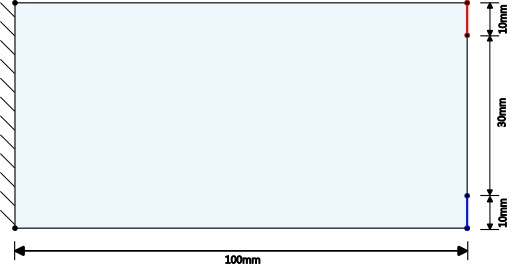
\includegraphics[width=0.8\linewidth]{figures/chapter_6/Case1Domain.png}
    \caption{Test Case One Domain with a thermal load (red) and structural load (blue)}
    \label{fig:test_case_one_domain}
\end{figure}

Figure \ref{fig:test_case_one_pareto_front} shows the obtained Pareto front for this setup. Despite the fact that the two boundary conditions were intended to be competing, it turns out they contribute to each other, as is observed in the Pareto front for the weights between $w=0.25$ to $w=0.75$ are close to each other.
\begin{figure}[ht]
    \centering
    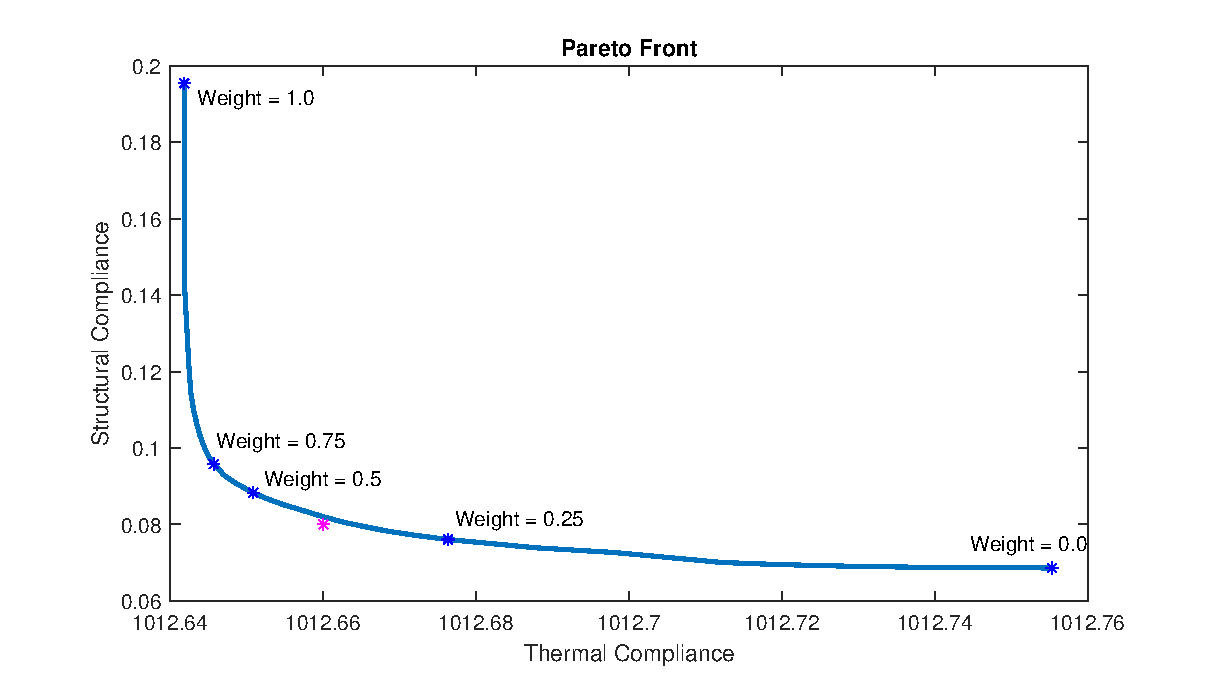
\includegraphics[width=0.6\linewidth]{figures/chapter_6/Case2_ParetoFront.eps} 
    \caption{Pareto front for test case one showing the chosen utopia point (magenta)}
    \label{fig:test_case_one_pareto_front}
\end{figure}

Figure \ref{fig:test_case_one_structures} shows some optimal structures that were recorded. The structure optimized for a weight of $w=0.5$ shows that although the boundary conditions are not aligned, the generated structure produces a shape that allows the two boundary conditions to assist each other in minimizing the total objective function.
\begin{figure}[ht]
    \begin{subfigure}[b]{0.3\linewidth}
        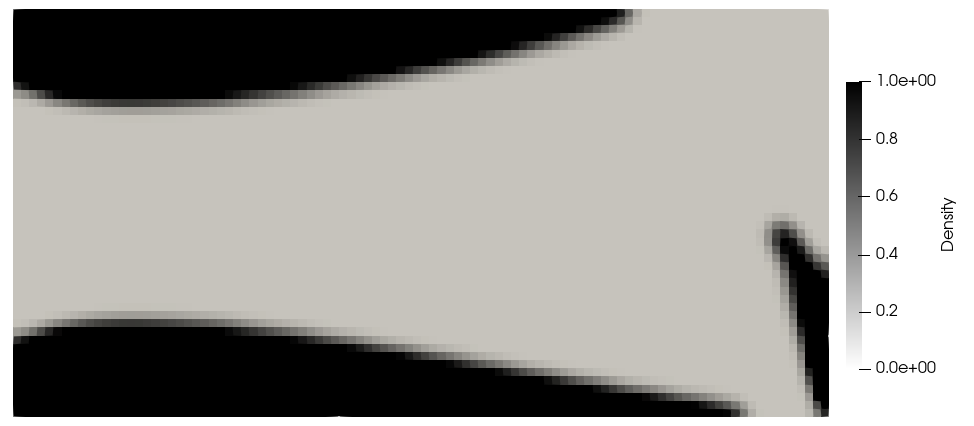
\includegraphics[width=\linewidth]{figures/chapter_6/Case2_MF_0to1.png}
        \caption{Optimized structure for \\$w=0.0$}
    \end{subfigure}
    \hfill
    \begin{subfigure}[b]{0.3\linewidth}
        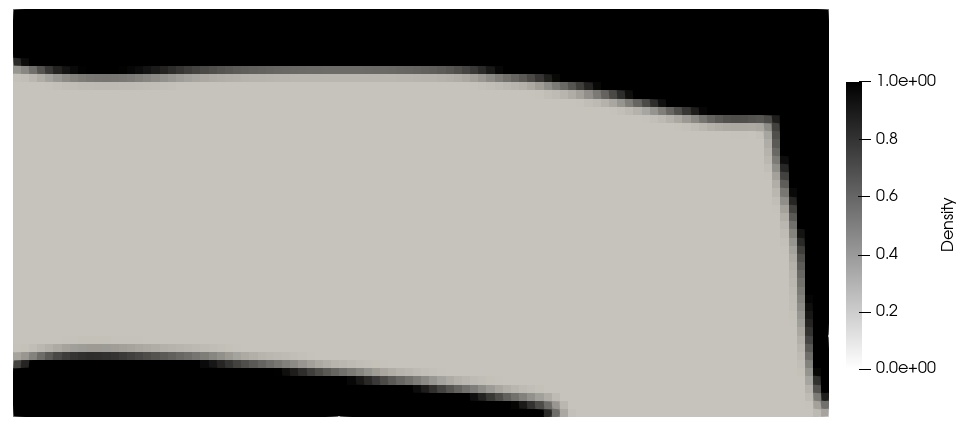
\includegraphics[width=\linewidth]{figures/chapter_6/Case2_MF_1to1.png}
        \caption{Optimized structure for \\$w=0.5$}
    \end{subfigure}
    \hfill
    \begin{subfigure}[b]{0.3\linewidth}
        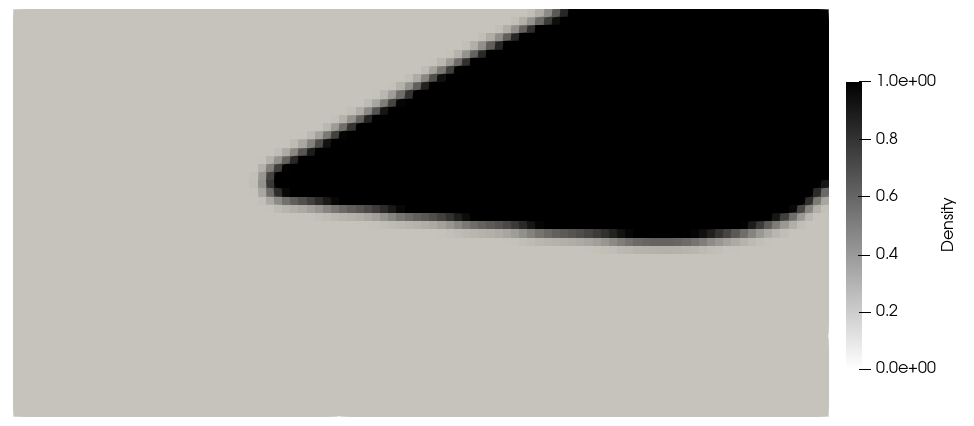
\includegraphics[width=\linewidth]{figures/chapter_6/Case2_MF_1to0.png}
        \caption{Optimized structure for \\$w=1.0$}
    \end{subfigure}
    \caption{Optimized structures for test case one}
    \label{fig:test_case_one_structures}
\end{figure}

Figure \ref{fig:test_case_one_pareto_optimum} shows the Pareto optimal point determined for the utopia point $U(312.6,0.01)$. Under these boundary conditions, the developed algorithm had no issues converging to the selected utopia point, even though the error norm plot has quite a wide well. The optimal point was found in just two iterations due to the initial guess being so accurate.
\begin{figure}[ht]
    \centering
    \hfill
    \begin{subfigure}[b]{0.45\linewidth}
        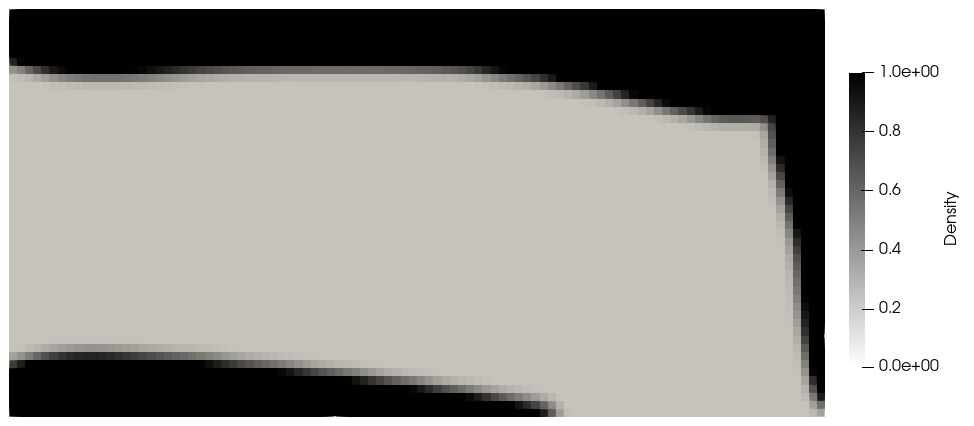
\includegraphics[width=\linewidth]{figures/chapter_6/Case1_ParetoOptimum.png}
        \caption{Pareto optimal structure}
    \end{subfigure}
    \hfill
    \begin{subfigure}[b]{0.25\linewidth}
        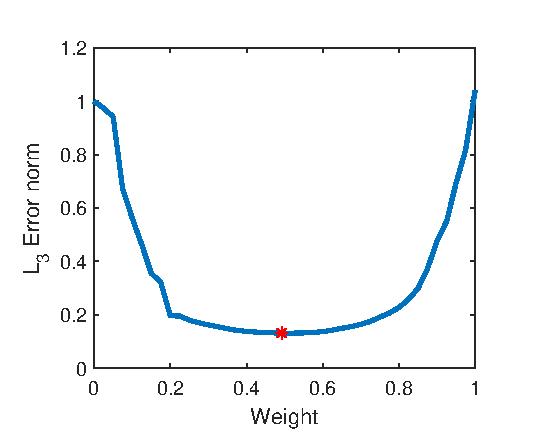
\includegraphics[width=\linewidth]{figures/chapter_6/Case1_ErrorNormPlot.eps}
        \caption{Error norm plot}
    \end{subfigure}
    \hfill
    \caption{Optimal structure obtained for utopia point $U(312.6,0.01)$ (left) as well as the error norm plot (right) produced for verification}
    \label{fig:test_case_one_pareto_optimum}
\end{figure}


\section{Case Two}
Test case two has been designed to test different boundary conditions. The bottom left node is fixed, while the bottom right node can slide in the x direction. A large distributed load across the top of the domain is also used. The thermal boundary condition is placed along the bottom in the center, meaning these boundary conditions should contribute to each other for the overall goal function.
\begin{figure}[ht]
    \centering
    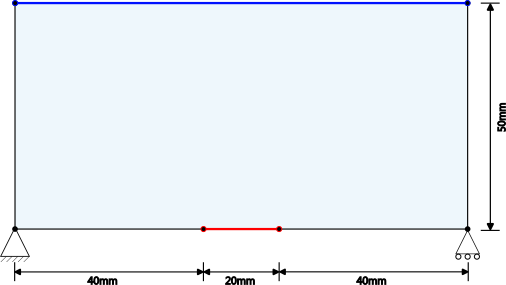
\includegraphics[width=0.8\linewidth]{figures/chapter_6/Case2Domain.png}
    \caption{Test Case Two Domain}
    \label{fig:test_case_two_domain}
\end{figure}

Figure \ref{fig:test_case_two_pareto_front} shows the Pareto front obtained for the boundary conditions of this case. It turns out that the boundary conditions partially compete with each other, unlike what was hypothesized. This occurs because as the thermal optimum develops, it removes a significant amount of material from where it is needed for the structural optimum. 
\begin{figure}[ht]
    \centering
    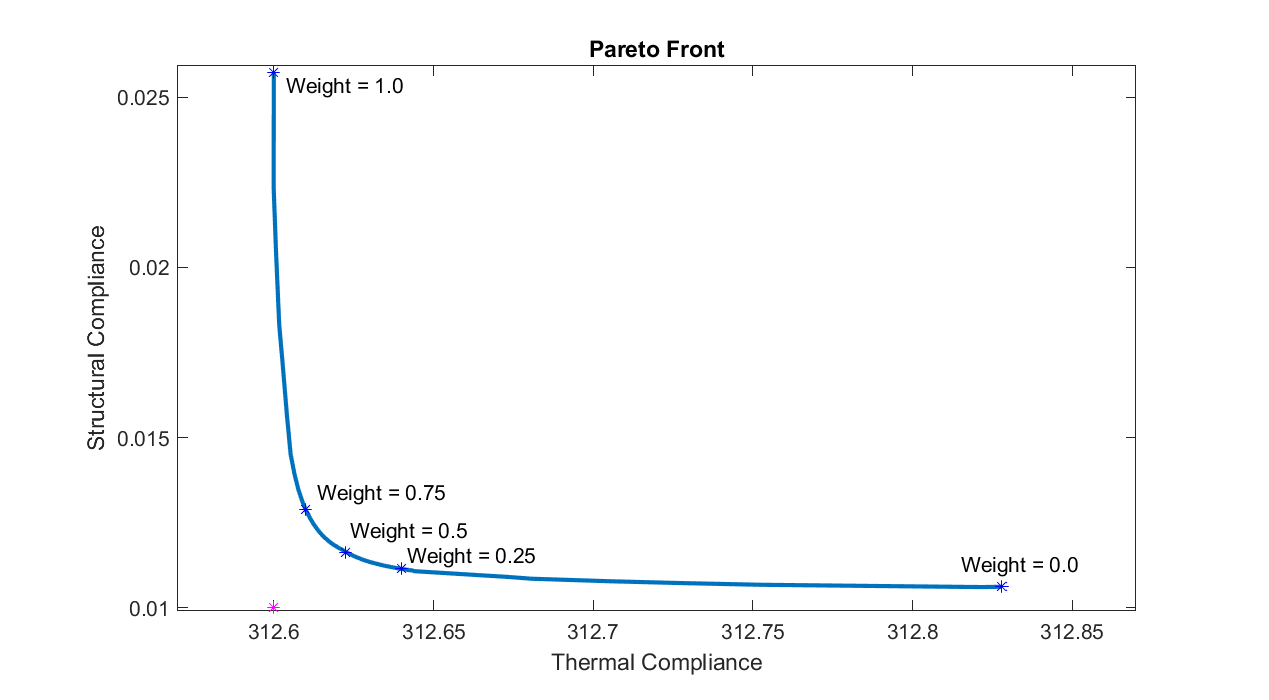
\includegraphics[width=0.6\linewidth]{figures/chapter_6/Case1_ParetoFront.eps} 
    \caption{Pareto front for test case two showing the chosen utopia point (magenta)}
    \label{fig:test_case_two_pareto_front}
\end{figure}

Figure \ref{fig:test_case_two_structures} also shows some optimal structures that were generated. They show that the thermal optimum essentially grows from the structural optimum. This backs up the idea that the two boundary conditions contribute to each other.
\begin{figure}[ht]
    \begin{subfigure}[b]{0.3\linewidth}
        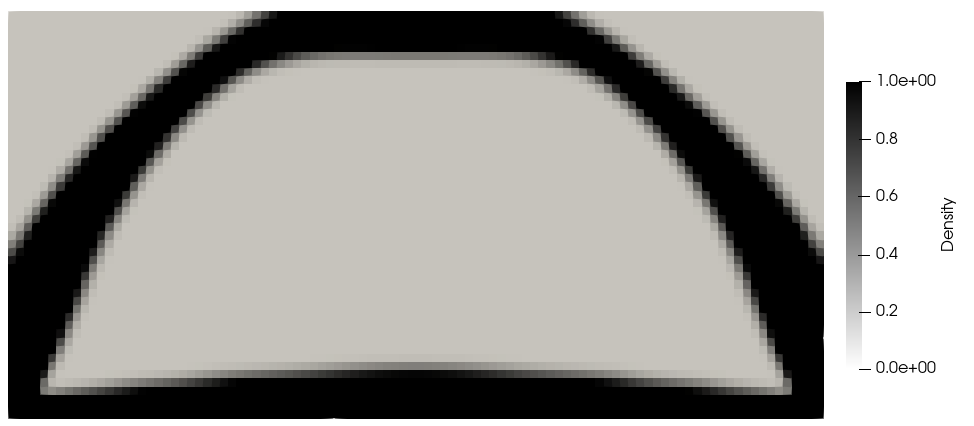
\includegraphics[width=\linewidth]{figures/chapter_6/Case1_MF_0to1.png}
        \caption{Optimized structure for \\$w=0.0$}
    \end{subfigure}
    \hfill
    \begin{subfigure}[b]{0.3\linewidth}
        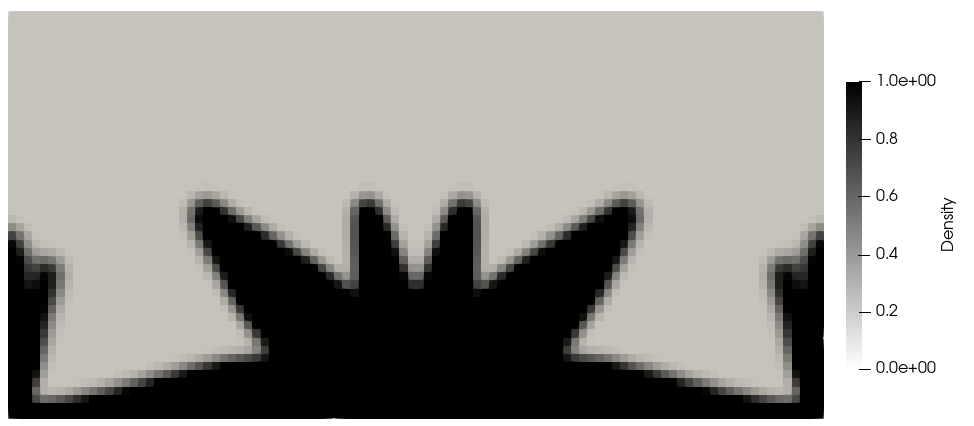
\includegraphics[width=\linewidth]{figures/chapter_6/Case1_MF_1to1.png}
        \caption{Optimized structure for \\$w=0.5$}
    \end{subfigure}
    \hfill
    \begin{subfigure}[b]{0.3\linewidth}
        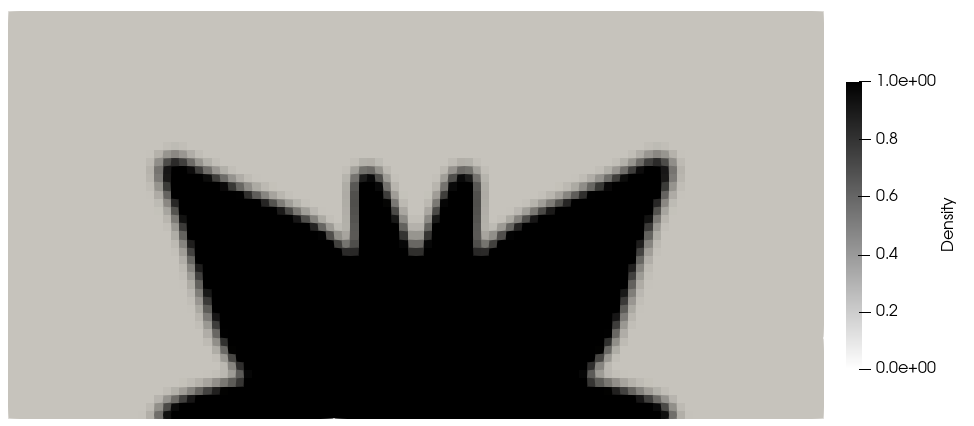
\includegraphics[width=\linewidth]{figures/chapter_6/Case1_MF_1to0.png}
        \caption{Optimized structure for \\$w=1.0$}
    \end{subfigure}
    \caption{Optimized structures for test case two}
    \label{fig:test_case_two_structures}
\end{figure}

Figure \ref{fig:test_case_two_pareto_optimum} shows the optimized structure and error norm plot. Again, the minimum error is found quite easily due to a sharpening towards the optimum. Even though these are simple boundary conditions, this result in particular shows that error and Pareto front aren't always going to produce results that are expected. This test case also shows that the boundary conditions that should contribute to each other can end up competing when they are too far apart. Too much material is required by each separate function which results in one function, in this case, the thermal function, dominating the kind of structure that can form. The optimum was determined within a good tolerance in five iterations but fully converged in nine.
\begin{figure}[ht]
    \centering
    \hfill
    \begin{subfigure}[b]{0.45\linewidth}
        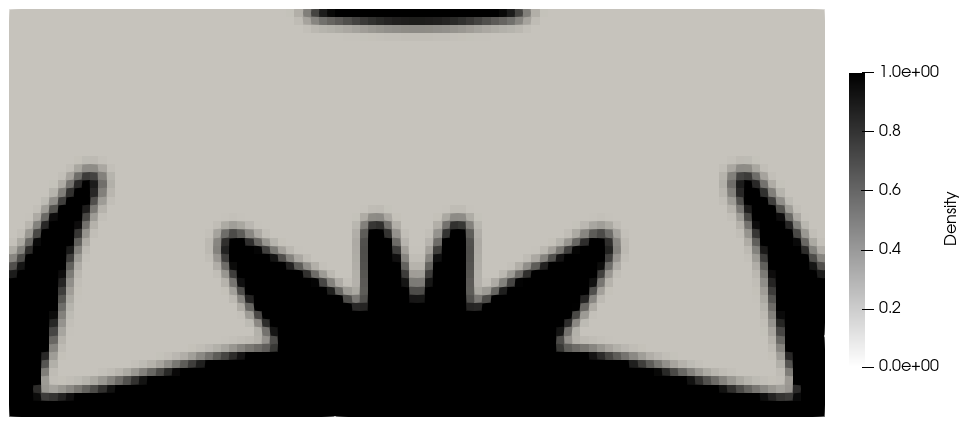
\includegraphics[width=\linewidth]{figures/chapter_6/Case2_ParetoOptimum.png}
        \caption{Pareto optimal structure}
    \end{subfigure}
    \hfill
    \begin{subfigure}[b]{0.25\linewidth}
        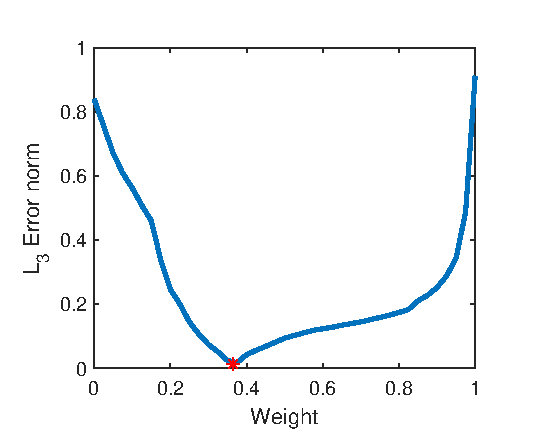
\includegraphics[width=\linewidth]{figures/chapter_6/Case2_ErrorNormPlot.eps}
        \caption{Error norm plot}
    \end{subfigure}
    \hfill
    \caption{Optimal structure obtained for utopia point $U(312.6,0.01)$ (left) as well as the error norm plot (right) produced for verification}
    \label{fig:test_case_two_pareto_optimum}
\end{figure}


\section{Case Three}
Test case three has been designed as an extension to test case two to ensure that expected results are obtained for asymmetric boundary conditions. Based on the results from test cases one and two, it is expected that the boundary conditions contribute to each other than in case two. This is because they already partially contribute, but in this case, the material can be distributed closer to each boundary condition so that neither function can be dominant.
\begin{figure}[ht]
    \centering
    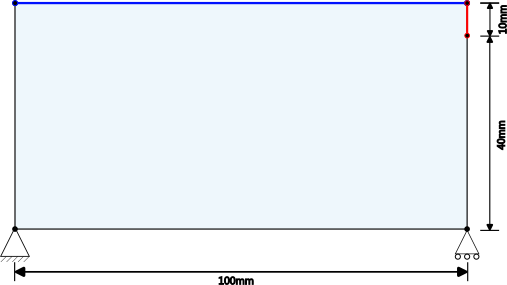
\includegraphics[width=0.7\linewidth]{figures/chapter_6/Case3Domain.png}
    \caption{Test Case Three Domain}
    \label{fig:test_case_three_domain}
\end{figure}

Figure \ref{fig:test_case_three_pareto_front} shows the Pareto front obtained for this final test case. Again the weights between $w=0.25$ and $w=0.75$ are close to each other because, as mentioned in this section's opening, the two boundary conditions contribute to each other. In fact, these two boundary conditions contribute so well with each other that between the weights $w=0.0$ to $w=0.25$ and $w=0.75$ to $w=1.0$, weakly Pareto optimal points are essentially found.
\begin{figure}[ht]
    \centering
    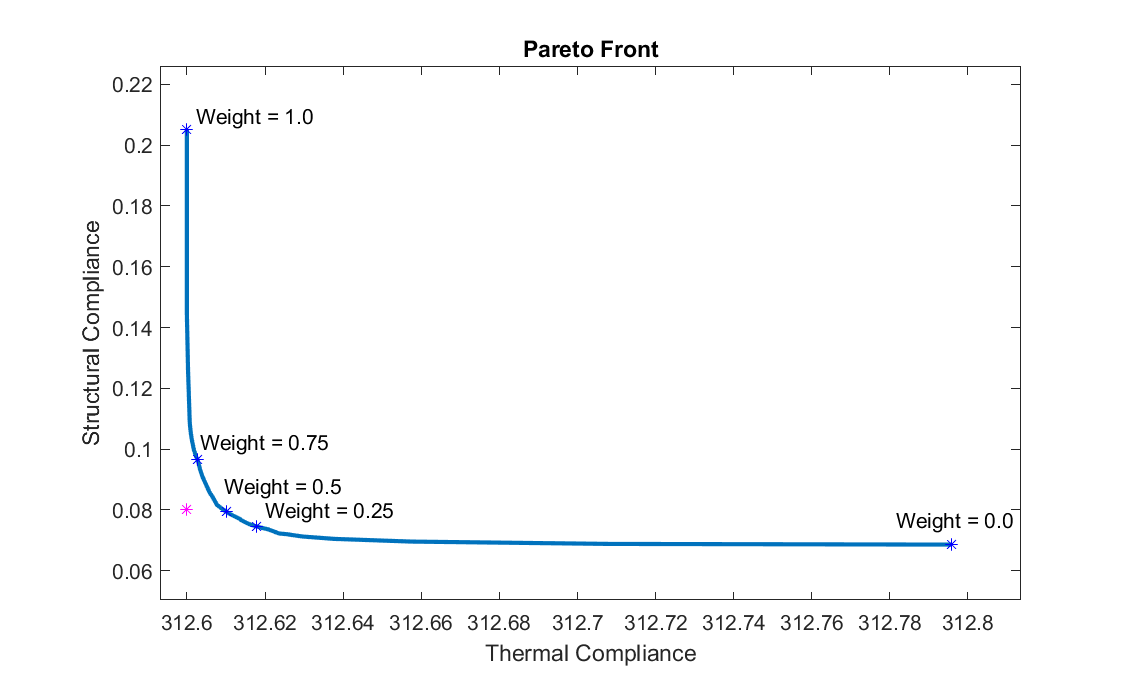
\includegraphics[width=0.6\linewidth]{figures/chapter_6/Case3_ParetoFront.eps} 
    \caption{Pareto front for test case three showing the chosen utopia point (magenta)}
    \label{fig:test_case_three_pareto_front}
\end{figure}

Figure \ref{fig:test_case_three_structures} shows how the two boundary conditions contribute to each other, especially on the right-hand side of the domain. They contribute because the thermal boundary condition allows the material to remain where it is required by the structural optimum on the right of the domain. This contrasts with case 2 which uniformly removed material from the top of the domain, limiting the structural compliance.
\begin{figure}
    \begin{subfigure}[b]{0.3\linewidth}
        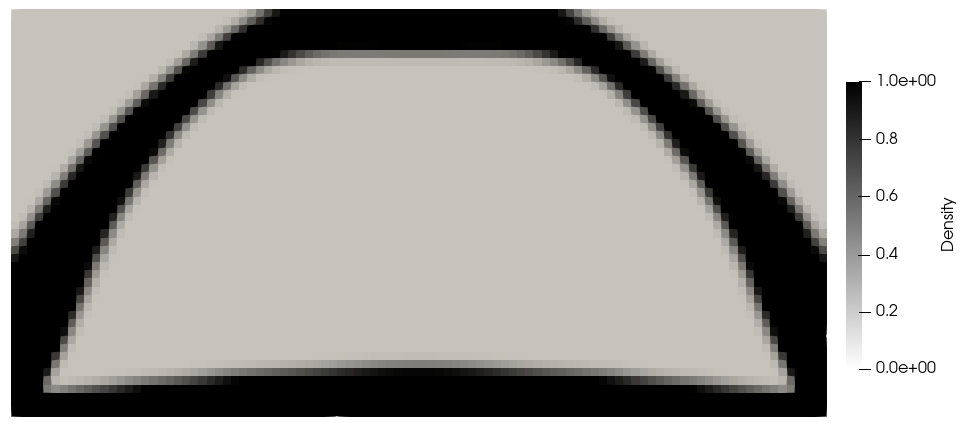
\includegraphics[width=\linewidth]{figures/chapter_6/Case3_MF_0to1.png}
        \caption{Optimized structure for \\$w=0.0$}
    \end{subfigure}
    \hfill
    \begin{subfigure}[b]{0.3\linewidth}
        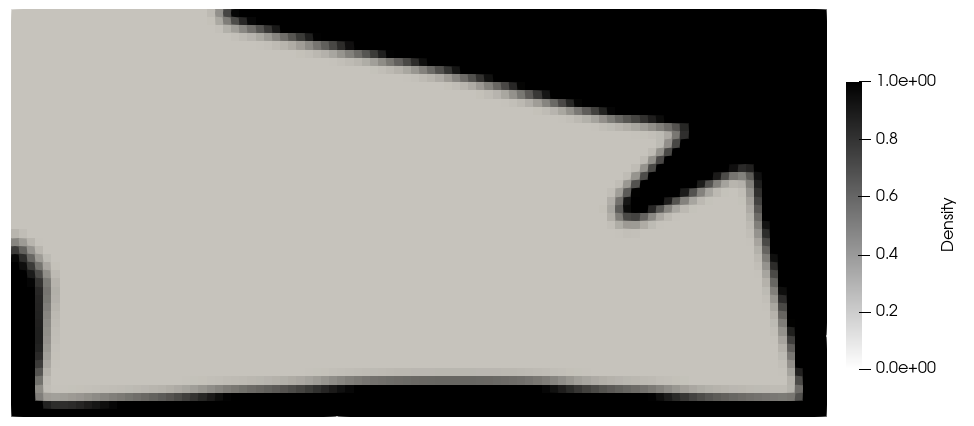
\includegraphics[width=\linewidth]{figures/chapter_6/Case3_MF_1to1.png}
        \caption{Optimized structure for \\$w=0.5$}
    \end{subfigure}
    \hfill
    \begin{subfigure}[b]{0.3\linewidth}
        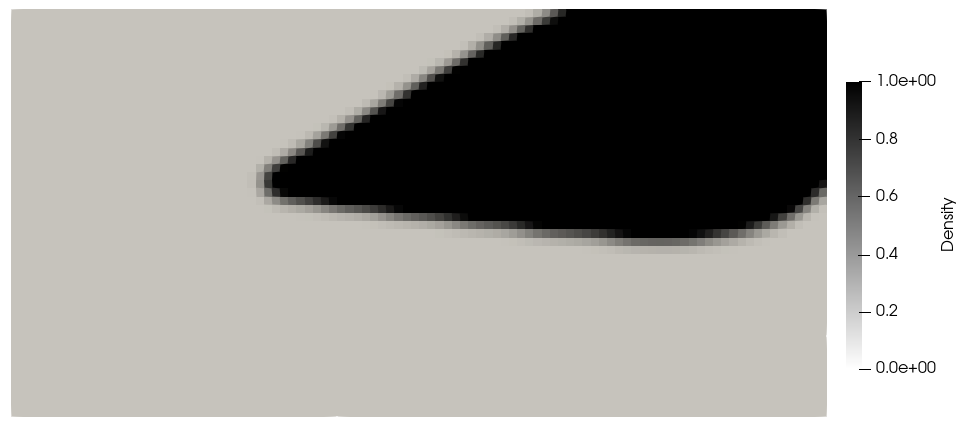
\includegraphics[width=\linewidth]{figures/chapter_6/Case3_MF_1to0.png}
        \caption{Optimized structure for \\$w=1.0$}
    \end{subfigure}
    \caption{Optmized structures for test case three}
    \label{fig:test_case_three_structures}
\end{figure}

Figure \ref{fig:test_case_three_pareto_optimum} shows the optimized structure and error norm plot. In this case, the minimum is close, but not exactly the minimum. The initial guess was good, but the algorithm converged too slowly. The error is still within a reasonable tolerance, but improvements should be made to ensure a true global minimum can be found.
\begin{figure}[ht]
    \centering
    \hfill
    \begin{subfigure}[b]{0.5\linewidth}
        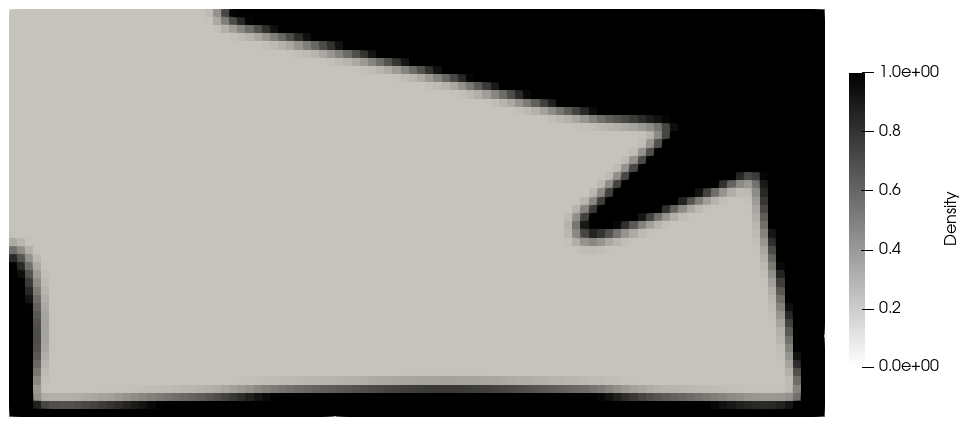
\includegraphics[width=\linewidth]{figures/chapter_6/Case3_ParetoOptimum.png}
        \caption{Pareto optimal structure}
    \end{subfigure}
    \hfill
    \begin{subfigure}[b]{0.3\linewidth}
        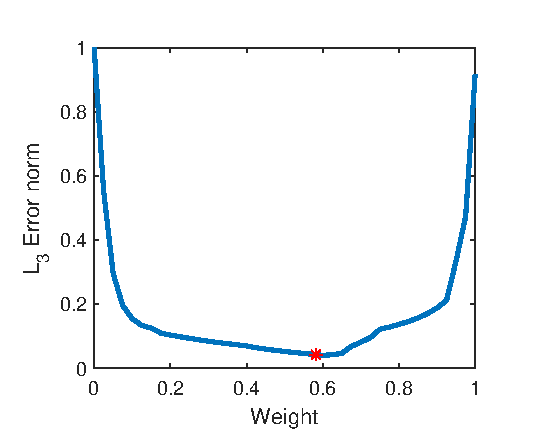
\includegraphics[width=\linewidth]{figures/chapter_6/Case3_ErrorNormPlot.eps}
        \caption{Error norm plot}
    \end{subfigure}
    \hfill
    \caption{Optimal structure obtained for utopia point $U(312.6,0.01)$ (left) as well as the error norm plot (right) produced for verification}
    \label{fig:test_case_three_pareto_optimum}
\end{figure}


\section{Remarks}
Of the boundary conditions that were devised, all produced a convex Pareto-front. As the algorithm is sensitive to the initial guess, this information can be useful when trying to determine the initial weight. Instead of projecting the point onto a line segment, the point could instead be projected onto the reciprocal function $y=k/x$, where $k$ can be used to control how sharp the shape of the curve is. The most generic form of this function is given in equation \ref{eq:recipricol_function_generic}.
\begin{equation}
    y = \frac{k}{x+a} + b
    \label{eq:recipricol_function_generic}
\end{equation}

The variables $a$ and $b$ are used to shift the function. They can be determined by solving a pair of simultaneous equations. If $y$ is the normalized compliance of the first function, and $x$ for the second, then a system of simultaneous can be determined as shown in equation \ref{eq:recipicol_simultaneous_equations}.
\begin{equation}
    \begin{split}
        \frac{k}{a} + b &= 1 \\
        \frac{k}{1 + a} + b &= 0
    \end{split}
    \label{eq:recipicol_simultaneous_equations}
\end{equation}

By rearranging the second equation, an equation for $b$ can be found which can then be used to determine $a$ using the quadratic formula, as shown in equation \ref{eq:recipicol_solved}.
\begin{equation}
    \begin{split}
        b &= \frac{k}{1 + a} \\
        a &= \frac{-1 + \sqrt{1 + 4k}}{2}
    \end{split}
    \label{eq:recipicol_solved}
\end{equation}

With that, the utopia point, $U$, can be projected onto the curve by defining the goal function shown in equation \ref{eq:goal_function}. The value $x$ can be determined using a gradient descent or similar method.
\begin{equation}
    \text{argmin}_{x\in[0,1]} \lVert (y,x) - U\rVert _p
    \label{eq:goal_function}
\end{equation}

\begin{figure}[ht]
    \centering
    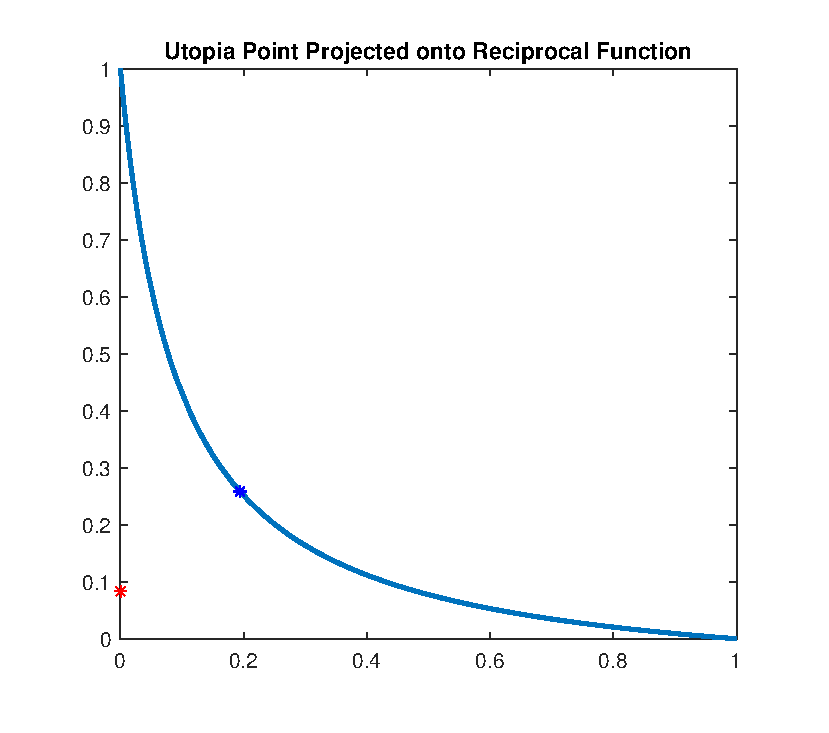
\includegraphics[width=0.5\linewidth]{figures/chapter_6/ProjectionIdea.eps}
    \caption{Projection (blue) of utopia point (magenta) onto the reciprocal function (blue line)}
\end{figure}

Once $x$ has been determined, the distance along the curve from $x=0$ needs to be determined. It is this distance that corresponds to the weight. This can be found by solving equation \ref{eq:distance_along_curve}. This method assumes the weights to be even distributed along the curve, which is generally not the case. This approach could be modified with a weighting function to reduce the calculated \emph{distance} along the curve near the endpoints.
\begin{equation}
    S(x) = \frac{1}{S(1)} \int_0^x \sqrt{(1 + \left(\frac{dy}{dx}\right)^2)} \ dt 
    \label{eq:distance_along_curve}
\end{equation}

To resolve the issue discussed in case 3, the quadratic fit method could be accelerated by considering gradient information obtained by previous iterations. A gradient descent sub-step could be performed to improve convergence in shallow wells. However, certain checks would need to be performed to ensure minimal overshooting occurs.